% === Begin Label Data ===
% ID: 835
% 难度星级: 
% 标签: 
% 备注: 
% 组卷引用次数: 0
% === End  Label Data ===

\begin{problem}{2022}{G}{全国甲卷（理）}{16}{解三角形}
已知 $\triangle ABC$ 中，点 $D$ 在边 $BC$ 上，$\angle ADB = 120^\circ$，$AD = 2$，$CD = 2BD$．当 $\dfrac{AC}{AB}$ 取得最小值时，$BD = \sqrt{3} - 1$．
\end{problem}

\begin{answer}
$\sqrt{3} - 1$
\end{answer}

\begin{solutions}
将 $\triangle ABD$ 沿 $AD$ 翻折得到 $\triangle AED$ . 

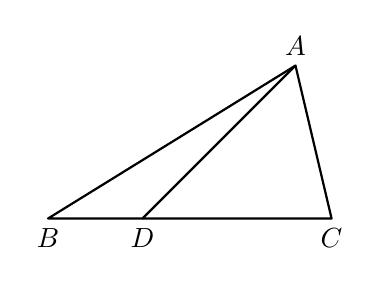
\begin{tikzpicture}[line cap=round,line join=round,scale=0.6]
\pgfmathsetmacro{\sfive}{sqrt(5)}

\coordinate (B) at (-3,0);
\coordinate (C) at (3,0);
\coordinate (D) at (-1,0);                % BD:DC=1:2
\coordinate (A) at (\sfive,{1+\sfive});   % 取一个合适位置（示意）

\draw[thick] (B)--(C)--(A)--cycle;
\draw[thick] (A)--(D);

\node[below] at (B) {$B$};
\node[below] at (D) {$D$};
\node[below] at (C) {$C$};
\node[above] at (A) {$A$};
\end{tikzpicture}

因此 $ BD = DE$，$\angle BDE = 120^\circ$，因此 $ \angle EBD = 30^\circ$，且 $BC = 3BD = \sqrt{3}BE$ .
 
因此 $ EB = EC$，由托勒密定理知 $AB \cdot EC + AC \cdot BE \geq AE \cdot BC$ . 

因此 $ \dfrac{AC}{AB} \geq \sqrt{3} - 1$，当 $A$、$B$、$E$、$C$ 四点共圆时取得等号即 $\dfrac{AC}{AB}$ 取得最小值 . 

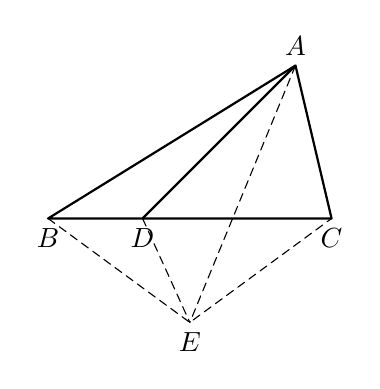
\begin{tikzpicture}[line cap=round,line join=round,scale=0.6]
\pgfmathsetmacro{\sfive}{sqrt(5)}

\coordinate (B) at (-3,0);
\coordinate (C) at (3,0);
\coordinate (D) at (-1,0);
\coordinate (A) at (\sfive,{1+\sfive});

% E 取在下方（示意折叠后的点）
\coordinate (E) at (0,-2.2);

\draw[thick] (B)--(C)--(A)--cycle;
\draw[thick] (A)--(D);

\draw[densely dashed] (B)--(E)--(C);
\draw[densely dashed] (D)--(E);
\draw[densely dashed] (A)--(E);

\node[below] at (B) {$B$};
\node[below] at (D) {$D$};
\node[below] at (C) {$C$};
\node[above] at (A) {$A$};
\node[below] at (E) {$E$};
\end{tikzpicture}

作 $\triangle ABC$ 外接圆，圆心为 $O$ 恰在 $AD$ 上  

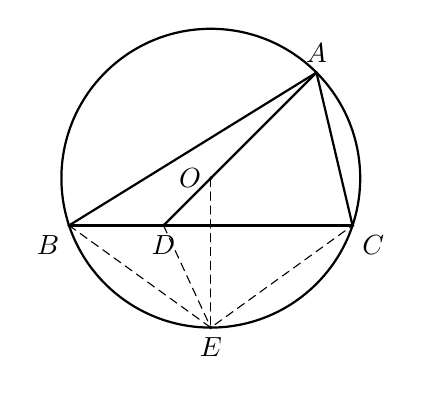
\begin{tikzpicture}[line cap=round,line join=round,scale=0.6]
\pgfmathsetmacro{\sfive}{sqrt(5)}
\pgfmathsetmacro{\R}{sqrt(10)}

\coordinate (B) at (-3,0);
\coordinate (C) at (3,0);
\coordinate (D) at (-1,0);
\coordinate (O) at (0,1);                 % 让 O 在 AD 上（按构造选取）
\coordinate (A) at (\sfive,{1+\sfive});   % 同时保证 A,B,C 共圆（圆心 O，半径 sqrt(10)）
\coordinate (E) at (0,{1-\R});            % 圆的最低点（示意）

\draw[thick] (O) circle (\R);

\draw[thick] (B)--(C);
\draw[thick] (A)--(B);
\draw[thick] (A)--(C);
\draw[thick] (A)--(D);

\draw[densely dashed] (B)--(E)--(C);
\draw[densely dashed] (D)--(E);
\draw[densely dashed] (O)--(E);

\fill (A) circle (1.1pt);
\fill (B) circle (1.1pt);
\fill (C) circle (1.1pt);
\fill (D) circle (1.1pt);
\fill (E) circle (1.1pt);
\fill (O) circle (1.1pt);

\node[above] at (A) {$A$};
\node[below left] at (B) {$B$};
\node[below right] at (C) {$C$};
\node[below] at (D) {$D$};
\node[below] at (E) {$E$};
\node[left] at (O) {$O$};
\end{tikzpicture}

$OA = OC = \sqrt{3}OD$，因此 $ BD = OD = \dfrac{AD}{\sqrt{3} + 1} = \sqrt{3} - 1$.

\end{solutions}